%%%%%%%%%%%%%%%%%%%%%%%%%%%%%%%%%%%%%%%%%%%%%%%%%%%%%%%%%%%%%%%%%%%%%%%%%%%%%%%%%%%%%%%%%%%%%%%%%%%%%%%%%
%%%%%%%%%%%%%%%%%%%%%%%%%%%%%%%%%%%%%%%%%%%% Header %%%%%%%%%%%%%%%%%%%%%%%%%%%%%%%%%%%%%%%%%%%%%%%%%%%%%
%%%%%%%%%%%%%%%%%%%%%%%%%%%%%%%%%%%%%%%%%%%%%%%%%%%%%%%%%%%%%%%%%%%%%%%%%%%%%%%%%%%%%%%%%%%%%%%%%%%%%%%%%

\documentclass[a4paper,titlepage,11pt,twosides,floatssmall]{mwrep}

\usepackage[left=2.5cm,right=2.5cm,top=2.5cm,bottom=2.5cm]{geometry} % Pages' geometry and layout
\usepackage[OT1]{fontenc} % Defines encoding for fonts (OT1 - original TeX encoding) 
\usepackage{polski} % Polish language specifics
\usepackage{amsmath} % Mathematical commands
\usepackage{amsfonts} % Fonts commands
\usepackage{amssymb} % Symbolical commands
\usepackage{graphicx} % Importing external graphics
\usepackage{float} % Forcing plot's position
\usepackage{url} % Web-related text (urls, mail adresses, etc.)
\usepackage{tikz} % Creating graphical elements like lines, dots, curves, figures
\usepackage{rotating} % Rotating objects of an arbitrary angle
\usepackage[percent]{overpic} % Makes it able to put LaTeX commands onto the included graphics (with a dedicated environment)
\usepackage[cp1250]{inputenc} % Non-standrard encoding of the LaTeX files
\usepackage{xcolor} % Easy driver-independent access to several kinds of color tints, shades, tones, and mixes of arbitrary colors
\usepackage{pgfplots} % High-quality function plots in normal or logarithmic scaling with a user-friendly interface
\usepackage{listings} % Source code printer
\usepackage{matlab-prettifier} % Matlab source code printer
\usepackage{enumitem} % List environments
\usepackage{siunitx} % Physical units
\usepackage{float} % force figure anchoring

% tikz packages choice
\usetikzlibrary{arrows,calc,decorations.markings,math,arrows.meta}
\usetikzlibrary{pgfplots.groupplots}

% siunitx settings
\sisetup{detect-weight,exponent-product=\cdot,output-decimal-marker={,},per-mode=symbol,binary-units=true,range-phrase={-},range-units=single}
\SendSettingsToPgf % unifies settings of the pgfplots package with siunitx package

% listings settings
\definecolor{gray}{rgb}{0.95,0.95,0.95}
\lstset{
	backgroundcolor=\color{gray},
	frame=single,
	breaklines=true,
}

% listings styles
\lstdefinestyle{customlatex}{
	basicstyle=\footnotesize\ttfamily,
	% basicstyle=\small\ttfamily,
}
\lstdefinestyle{customc}{
	breaklines=true,
	frame=tb,
	language=C,
	xleftmargin=0pt,
	showstringspaces=false,
	basicstyle=\small\ttfamily,
	keywordstyle=\bfseries\color{green!40!black},
	commentstyle=\itshape\color{purple!40!black},
	identifierstyle=\color{blue},
	stringstyle=\color{orange},
}
\lstdefinestyle{custommatlab}{
	captionpos=t,
	breaklines=true,
	frame=tb,
	xleftmargin=0pt,
	language=matlab,
	showstringspaces=false,
	% basicstyle=\footnotesize\ttfamily,
	basicstyle=\scriptsize\ttfamily,
	keywordstyle=\bfseries\color{green!40!black},
	commentstyle=\itshape\color{purple!40!black},
	identifierstyle=\color{blue},
	stringstyle=\color{orange},
}

% Text field size (without header and footer - bez "�ywej paginy")
\textwidth 160mm \textheight 247mm

% pgfplots settings
\pgfplotsset{
	tick label style={font=\scriptsize},
	label style={font=\small},
	legend style={font=\small},
	title style={font=\small}
}

\def\figurename{Rys.}
\def\tablename{Tab.}

% Max number of floating elements configuration
\setcounter{topnumber}{0} % default : 2
\setcounter{bottomnumber}{3} % default : 1
\setcounter{totalnumber}{5} % default : 3

\renewcommand{\textfraction}{0.01} % default : 0.2
\renewcommand{\topfraction}{0.95} % default : 0.7
\renewcommand{\bottomfraction}{0.95} % default : 0.3
\renewcommand{\floatpagefraction}{0.35} % default : 0.5


%%%%%%%%%%%%%%%%%%%%%%%%%%%%%%%%%%%%%%%%%%%%%%%%%%%%%%%%%%%%%%%%%%%%%%%%%%%%%%%%%%%%%%%%%%%%%%%%%%%%%%%%%
%%%%%%%%%%%%%%%%%%%%%%%%%%%%%%%%%%%%%% Document utilities %%%%%%%%%%%%%%%%%%%%%%%%%%%%%%%%%%%%%%%%%%%%%%%
%%%%%%%%%%%%%%%%%%%%%%%%%%%%%%%%%%%%%%%%%%%%%%%%%%%%%%%%%%%%%%%%%%%%%%%%%%%%%%%%%%%%%%%%%%%%%%%%%%%%%%%%%

% Title Page Data
\title{\bf Sprawozdanie z projektu nr 2 \\ zesp� nr 9\vskip 0.1cm}
\author{Pawe� Bugyi, Marcin Michalski, Krzysztof Pierczyk}
\date{2020}

% Maketitle macro
\makeatletter
\renewcommand{\maketitle}
{
	\begin{titlepage}
		\begin{center}{
			\LARGE {\bf
			Wydzia� Elektroniki i Technik Informacyjnych}}\\
			\vspace{0.4cm}
			{\LARGE {\bf Politechnika Warszawska}}\\
			\vspace{0.3cm}
		\end{center}
		\vspace{5cm}
		\begin{center}
			{\bf \LARGE Projektowanie uk�ad�w sterowania\\ (projekt grupowy) \vskip 0.1cm}
		\end{center}
		\vspace{1cm}
		\begin{center}
			{\bf \LARGE \@title}
		\end{center}
		\vspace{2cm}
		\begin{center}
			{\bf \Large \@author \par}
		\end{center}
		\vspace*{\stretch{6}}
		\begin{center}
			\bf{\large{Warszawa, \@date\vskip 0.1cm}}
		\end{center}
	\end{titlepage}
}
\makeatother

%%%%%%%%%%%%%%%%%%%%%%%%%%%%%%%%%%%%%%%%%%%%%%%%%%%%%%%%%%%%%%%%%%%%%%%%%%%%%%%%%%%%%%%%%%%%%%%%%%%%%%%%%
%%%%%%%%%%%%%%%%%%%%%%%%%%%%%%%%%%%%%%%%%%% Document %%%%%%%%%%%%%%%%%%%%%%%%%%%%%%%%%%%%%%%%%%%%%%%%%%%%
%%%%%%%%%%%%%%%%%%%%%%%%%%%%%%%%%%%%%%%%%%%%%%%%%%%%%%%%%%%%%%%%%%%%%%%%%%%%%%%%%%%%%%%%%%%%%%%%%%%%%%%%%

\begin{document}

% Pages' style formatting
\frenchspacing
\pagestyle{uheadings}

% Use maketitle macro to build title page
\maketitle

% Insert parts of the report
\tableofcontents
\chapter{Wst�p}
Drugi projekt z~Projektowania Uk�ad�w Sterowania (PUST) stanowi� rozszerzenie projektu pierwszego. Ponownie zaj�li�my si� badaniem obiektu, danego funkcj� napisan� w Matlabie oraz projektowaniem i strojeniem do niego uk�adu regulacji. Rozszerzenie polega�o na przej�ciu z~obiektu typu SISO (\textit{ang.} Single-input-single-output) na obiekt typu MISO (\textit{ang.} Multiple-input-\\single-output), w~kt�rym jedno z wej�� by�o wej�ciem niesterowanym (zak��ceniem procesu). Modyfikacja ta pozwoli�a nam na zweryfikowanie efektywno�ci algorytmu regulacji predykcjynej DMC ((\textit{ang.} Dynamic Matrix Control) przystosowanego do pracy z mierzalnym zak��ceniem. Niniejsze sprawozdanie stanowi podsumowanie ca�ego naszego trudu, wszystkich wylanych �ez, nieprzespanych nocy oraz pobitych element�w zastawy domowej zwi�zanych z realizacj� projektu.
\chapter{Badanie poprawno�ci punktu pracy}

Pierwsze zadanie sprowadza�o si� do zweryfikowania poprawno�ci, podanego w~tre�ci zadania, punktu pracy $U_{pp}=\num{1.7}$, $Y_{pp}=\num{2}$. Weryfikacja polega�a na podaniu na wej�cie obiektu sta�ej warto�ci pobudzenia $U=\num{1.7}$ przy jednoczesnym za�o�eniu, �e warto�� wyj�cia w~przesz�o�ci ustalona by�a na poziomie $Y=\num{2.0}$ i sprawdzeniu, czy warto�� ta ulegnie zmianie. Wynik eksperymentu zosta� przedstawiony na rys. \ref{work_point_check}. Zgodnie z~danymi podanymi w~tre�ci zadania, punkt $U=\num{1.7},Y=\num{2}$ jest rzeczywi�cie punktem pracy.

\vskip 0.5cm
\begin{figure}[h]
    \centering
        \begin{tikzpicture}
            \begin{axis}[
                    width=0.5\textwidth,
                    xmin=0,xmax=100,ymin=0,ymax=3,
                    xlabel={$t [s]$},
                    ylabel={$y(t)$},
                    xtick={0, 25, 50, 75, 100},
                    ytick={0,0.5,1.0,1.5, 2.0, 2.5, 3.0},
                    legend pos=south east,
                    y tick label style={/pgf/number format/1000 sep={,}},
                ]
                \addplot[const plot, blue]                file {data/exercise_1/work_point_check.txt};
                \legend{$y(t)$}
            \end{axis}
        \end{tikzpicture}
    \caption{Przebieg warto�ci wyj�ciowej procesu po podaniu sta�ego wej�cia $U=\num{1.7}$}
    \label{work_point_check}
\end{figure}
\vskip 0.5cm

\chapter{Wyznaczanie odpowiedzi skokowej}

Drugie zadanie polega�o na wyznaczeniu odpowiedzi uk�adu na kilka skokowych zmian warto�ci sygna�u steruj�cego przy zachowaniu ogranicze� ich warto�ci. Sygna� steruj�cy musi zawiera� si� w~przedziale $U\in[\num{1.4}; \num{2.0}]$. �rodkowi tego przedzia�u odpowiada punkt pracy uk�adu weryfikowany w~zadaniu nr 1, kt�ry w~tym przypadku pos�u�y� jako warto�� startowa. Obiekt zosta� doprowadzony do punktu pracy poprzez zainicjalizowanie wektor�w warto�ci steruj�cej i~warto�ci wyj�ciowej odpowiednimi warto�ciami $U=\num{1.7},Y=\num{2}$, co zosta�o przedstawione na poni�szym listingu.

\vskip 0.5cm
\begin{lstlisting}[style=Matlab-editor]
    U_init = ones(STEPS_NUM,1) * 1.7;
    Y_init = ones(STEPS_NUM,1) * 2;
\end{lstlisting} 
\vskip 0.5cm

Wykonano ��cznie 8 skok�w warto�ci steruj�cej, przy czym cztery z~nich mia�y warto�ci ujemne, a~cztery warto�ci dodatnie. Wszystkie zosta�y r�wno rozmieszczone pomi�dzy punktem pocz�tkowym, a~minimaln�/maksymaln� dozwolon� warto�ci�. Wyniki pomiar�w przedstawiono na rys. \ref{step_responses}. Dane pomiarowe zosta�y przesuni�te w~czasie tak, aby punkt pocz�tkowy ($Czas=0s$) by� momentem wykonania skoku sterowania.

\vskip 1cm
\begin{figure}[h]
    \centering
        \begin{tikzpicture}
            \begin{axis}[
                    width=0.5\textwidth,
                    xmin=0,xmax=100,ymin=1.5,ymax=2.5,
                    xlabel={$t [s]$},
                    ylabel={$y(t)$},
                    xtick={0,25,50,75,100},
                    ytick={1.5, 1.6, 1.7, 1.8, 1.9, 2.0, 2.1, 2.2, 2.3, 2.4, 2.5},
                    legend pos=south east,
                    legend style={font=\tiny},
                    y tick label style={/pgf/number format/1000 sep={,}},
                ]
                
                \addplot[const plot, blue]               file {data/exercise_2/step_response_1.txt};
                \addplot[const plot, cyan]               file {data/exercise_2/step_response_2.txt};
                \addplot[const plot, green]              file {data/exercise_2/step_response_3.txt};
                \addplot[const plot, lime]               file {data/exercise_2/step_response_4.txt};
                \addplot[const plot, olive]              file {data/exercise_2/step_response_5.txt};
                \addplot[const plot, yellow]             file {data/exercise_2/step_response_6.txt};
                \addplot[const plot, orange]             file {data/exercise_2/step_response_7.txt};
                \addplot[const plot, red]                file {data/exercise_2/step_response_8.txt};

                \legend{$\Delta U=\num{0.3}$,$\Delta U=\num{0.225}$,$\Delta U=\num{0.150}$,$\Delta U=\num{0.075}$,$\Delta U=\num{-0.075}$,$\Delta U=\num{-0.150}$,$\Delta U=\num{-0.225}$,$\Delta U=\num{-0.3}$}

            \end{axis}
        \end{tikzpicture}
    \caption{Przebieg warto�ci wyj�ciowej procesu przy skokowej zmianie sygna�u steruj�cego}
    \label{step_responses}
\end{figure}
\vskip 1cm

Druga cz�� zadania polega�a na zbadaniu charakterystyki statycznej uk�adu i~okre�leniu, czy proces jest w przybli�eniu liniowy. Zebrawszy odpowiedzi skokowe stworzyli�my wektor par $(U_{pp}, Y_{pp})$ reprezentuj�cych punkty pracy uk�adu. Punkty te wyrysowane na p�aszczy�nie ukaza�y charakterystyk�, kt�r� mo�emy obserwowa� na rys. \ref{static_characteristic}

\vskip 0.5cm
\begin{figure}[H]
    \centering
        \begin{tikzpicture}
            \begin{axis}[
                    width=0.5\textwidth,
                    xmin=1.4,xmax=2,ymin=1.5,ymax=2.5,
                    xlabel={$u$},
                    ylabel={$y(u)$},
                    xtick={1.4,1.5,1.6, 1.7, 1.8, 1.9, 2.0},
                    ytick={1.5, 1.6, 1.7, 1.8, 1.9, 2.0, 2.1, 2.2, 2.3, 2.4, 2.5},
                    legend pos=south east,
                    x tick label style={/pgf/number format/1000 sep={,}},
                    y tick label style={/pgf/number format/1000 sep={,}},
                ]
                \addplot[blue]                file {data/exercise_2/static_characteristic.txt};
            \end{axis}
        \end{tikzpicture}
    \caption{Charakterystyka statyczna obiektu}
    \label{static_characteristic}
\end{figure}
\vskip 0.5cm

Jak wida�, obiekt wykazuje silnie liniowy charakter. Pozwala to wyznaczy� wzmocnienie statyczne uk�adu, czyli warto�� zmiany wyj�cia uk�adu przy jednostkowej zmianie warto�ci sygna�u steruj�cego. Obliczaj�c stosunek zmiany na wyj�ciu uk�adu do zmiany warto�ci steruj�cej przy skoku z~$U=\num{1.7}$ do $U=\num{2.0}$ otrzymujemy r�wnanie pokazane na rys. \ref{static_gain}.

\vskip 0.5cm
\begin{equation}
    K = \dfrac{\Delta Y}{\Delta U} = \dfrac{\num{2.4320}}{\num{0.3}} = \num{0.6945}
    \label{static_gain}
\end{equation}
\vskip 0.5cm

\chapter{Wyznaczanie odpowiedzi skokowej do DMC}
Kolejnym krokiem do realizacji projektu by�o opracowanie wynik�w, otrzymanych w zadaniu drugim, i~uzyskanie z~nich odpowiedzi skokowej w~postaci wykorzystywanej w~algorytmie DMC. Bior�c pod uwag� wniosek dotycz�cy liniowo�ci obiektu w~ca�ym badanym zakresie, do tego celu wybra� mogli�my dowolne odpowiedzi skokowe z obu tor�w. Zdecydowali�my si� na skoki z~$u = 0$ do $u = 1$ oraz z~$z = 0$ do $z = 1$. Warto�� wej�ciowa toru komplementarnego by�a zerowa w~przypadku obydwu skok�w. Odpowiedzi te zosta�y przedstawione na rysunkach \ref{u_step_response} i \ref{z_step_response}.

\begin{figure}[h]
\centering
\begin{tikzpicture}
\begin{axis}[
width=0.5\textwidth,
xmin=0,xmax=190,ymin=0,ymax=3,
xlabel={$k$},
ylabel={$y(k)$},
legend pos=south east,
y tick label style={/pgf/number format/1000 sep=},
]
\addplot[red , semithick ] file { data/exercise_3/U_step_response_DMC.txt};
\legend{y(k)}
\end{axis}
\end{tikzpicture}
\caption{Odpowied� skokowa DMC na sygna� steruj�cy}
\label{u_step_response}
\end{figure}

\begin{figure}[h]
\centering
\begin{tikzpicture}
\begin{axis}[
width=0.5\textwidth,
xmin=0,xmax=40,ymin=0,ymax=2,
xlabel={$k$},
ylabel={$y(k)$},
legend pos=south east,
y tick label style={/pgf/number format/1000 sep=},
]
\addplot[red , semithick ] file { data/exercise_3/Z_step_response_DMC.txt};
\legend{y(k)}
\end{axis}
\end{tikzpicture}
\caption{Odpowied� skokowa DMC na zak��cenie}
\label{z_step_response}
\end{figure}

Liniowo�� obiektu i~brak ogranicze� warto�ci sygna��w pozwoli�y nam wybra� dogodne warto�ci skok�w co zniwelowa�o potrzeb� przeskalowywania otrzymanej odpowiedzi. Jedynym zabiegiem, jaki musieli�my wykona�, by�o wybranie z wektor�w pr�bek odpowiedzi tych, o~w�a�ciwych indeksach. Jako �e skoki odbywa�y si� w~chwili $n = 0$, do odpowiedzi skokowej zosta�y wzi�te tylko pr�bki z~chwil $n >= 1$. Wst�pne horyzonty dynamiki zosta�y wybrane tak, aby zmiana warto�ci wyj�cia w~chwilach $n > D$, gdzie $D$ to wybrany horyzont, by�y niewi�ksze ni� \num{0.01}\% warto�ci maksymalnej.

\chapter{DMC}
\section{Algorytm DMC w wersji MIMO}
Algorytm DMC w wersji MIMO dzia�a na tej samej zasadzie co algorytm DMC w wersji SISO, czyli oblicza zachowanie wyj�cia obiektu wprz�d na podstawie poprzednich przyrost�w sygna�u sterowania. Podstawowa r�nic� oczywi�cie jest to, �e w naszym przypadku jest 12 tor�w sterowania ( 4 wej�cia i 3 wyj�cia ), ale sama regu�a dzia�ania pozostaje taka sama. Ju� mo�na tutaj zauwa�y� przewag� DMC w wersji MIMO nad PID w wersji MIMO tak�, �e DMC wykorzystuje wszystkie wej�cia i "jest �wiadome" wp�ywu ka�dego wej�cia na ka�de wyj�cie. Pozwala to nam na otrzymanie znacz�co lepszej jako�ci regulacji co potwierdzaj� nasze eksperymenty. Oczywi�cie nie ma nic za darmo co oznacza, �e DMC w wersji MIMO wymaga znacz�co ilo�� oblicze� ni� PID w wersji MIMO, ale ten problem mo�emy zmniejszy� poprzez zaimplementowanie DMC w najprostszej wersji analitycznej ( dzi�ki temu mamy mniej oblicze� do wykonania co obr�t p�tli).

\section{Kalibracja algorytmu DMC w wersji MIMO}

Kalibracj� podzielili�my na dwie cz�ci. Pierwsza cz�� sk�ada si� z doboru parametr�w podstawowych takich jak horyzont dynamiki obiektu, horyzont predykcji i horyzont sterowania algorytmu DMC. Parametry Lambda i Psi s� r�wne 1, �eby nie faworyzowa� �adnego toru sterowania. Druga cz�� sk�ada si� z doboru parametr�w Lambda i Psi dla ustalonych wcze�niej warto�ci podstawowych.
	Dla otrzymania mo�liwie najlepszej jako�ci regulacji b�dziemy wykorzystawali wcze�niej wspomniany algorytm ewolucyjny, by mo�na por�wna� wyniki z wynikami regulacji za pomoc� algorytmu PID w wersji MIMO.
	
	Wyniki pierwszego etapu kalibracji mo�emy zobaczy� na wykresach poni�ej:
	
	\begin{center}
		\begin{figure}[H]
		\makebox[\textwidth]{\includegraphics[width=\paperwidth]{data/exercise_4_DMC/DMC_D_204_N_107_Nu_54_Lambda_1_1_1_1__Psi_1_1_1__U1_error_69.8736.pdf}}
		\label{DMC_D_204_N_107_Nu_54_Lambda_1_1_1_1__Psi_1_1_1__U1_error_69.8736}
		\caption{DMC=D=204, N=107, Nu=54, Lambda=[1, 1, 1, 1], [Psi=1, 1, 1], error=69.8736}
		\end{figure}
		\end{center}
	
	W drugim etapie kalibracji wykorzystamy zar�wno metod� in�ynierska jak i algorytm ewolucyjny, by m�c r�wnie� por�wna�, czy metoda in�ynierska pozwala na otrzymanie por�wnywalnego wyniku.
	Najpierw pragniemy pokaza� wyniki kalibracji metod� in�yniersk�:
	
	\begin{center}
		\begin{figure}[H]
		\makebox[\textwidth]{\includegraphics[width=\paperwidth]{data/exercise_4_DMC/DMC_D_204_N_107_Nu_54_Lambda_1_2_3_4__Psi_1_2_3__U1_error_69.2682.pdf}}
		\label{DMC_D_204_N_107_Nu_54_Lambda_1_2_3_4__Psi_1_2_3__U1_error_69.2682}
		\caption{DMC=D=204, N=107, Nu=54, Lambda=[1, 2, 3, 4], Psi=[1, 2, 3], error=69.2682}
		\end{figure}
		\end{center}

		\begin{center}
			\begin{figure}[H]
			\makebox[\textwidth]{\includegraphics[width=\paperwidth]{data/exercise_4_DMC/DMC_D_204_N_107_Nu_54_Lambda_0.5_0.5_0.5_0.5__Psi_1_1_1__U1_error_55.4869.pdf}}
			\label{DMC_D_204_N_107_Nu_54_Lambda_0.5_0.5_0.5_0.5__Psi_1_1_1__U1_error_55.4869}
			\caption{DMC=D=204, N=107, Nu=54, Lambda=[0.5, 0.5, 0.5, 0.5], Psi=[1, 1, 1], error=55.4869}
			\end{figure}
			\end{center}
			\begin{center}
				\begin{figure}[H]
				\makebox[\textwidth]{\includegraphics[width=\paperwidth]{data/exercise_4_DMC/DMC_D_204_N_107_Nu_54_Lambda_0.5_0.5_0.5_0.5__Psi_10_1_1__U1_error_45.7233.pdf}}
				\label{DMC_D_204_N_107_Nu_54_Lambda_0.5_0.5_0.5_0.5__Psi_10_1_1__U1_error_45.7233}
				\caption{DMC=D=204, N=107, Nu=54, Lambda=[0.5, 0.5, 0.5, 0.5], Psi=[10, 1, 1], error=45.7233}
				\end{figure}
				\end{center}

				\begin{center}
					\begin{figure}[H]
					\makebox[\textwidth]{\includegraphics[width=\paperwidth]{data/exercise_4_DMC/DMC_D_204_N_107_Nu_54_Lambda_0.5_0.5_0.5_0.5__Psi_20_1_1__U1_error_46.6045.pdf}}
					\label{DMC_D_204_N_107_Nu_54_Lambda_0.5_0.5_0.5_0.5__Psi_20_1_1__U1_error_46.6045}
					\caption{DMC=D=204, N=107, Nu=54, Lambda=[0.5, 0.5, 0.5, 0.5], Psi=[20, 1, 1], error=46.6045}
					\end{figure}
					\end{center}

	
	Jak wida� jako�� regulacji jest znacz�co lepsza ni� w przypadku algorytmu regulacji PID w wersji MIMO. B��d obliczany dla przyk�adowego przebiegu jest prawie 10-krotnie mniejszy ni� w przypadku PID.
	Teraz dla por�wnania wyniki algorytmu ewolucyjnego:
	
	\begin{center}
		\begin{figure}[H]
		\makebox[\textwidth]{\includegraphics[width=\paperwidth]{data/exercise_4_DMC/DMC_D_204_N_107_Nu_54_Lambda_42.7092_55.6008_357.2521_284.4598__Psi_503.0319_516.5173_980.2935__U1_error_45.2539.pdf}}
		\label{DMC_D_204_N_107_Nu_54_Lambda_42.7092_55.6008_357.2521_284.4598__Psi_503.0319_516.5173_980.2935__U1_error_45.2539}
		\caption{DMC=D=204, N=107, Nu=54, Lambda=[42.7092, 55.6008, 357.2521, 284.4598], Psi=[503.0319, 516.5173, 980.2935], error=45.2539}
		\end{figure}
		\end{center}
	
	Obliczony b��d na ca�ej d�ugo�ci przebiegu jest prawie taki sam jak z metody in�ynierskiej. Oznacza to, �e pomimo 7 parametr�w, kt�re na raz kalibrujemy jeste�my wstanie to zrobi� z wykorzystaniem do�wiadczenia zdobytego podczas kalibrowania innych regulator�w.

\chapter{Por�wnanie i wnioski}
\section{Por�wnianie wynik�w sterowania algorytmami PID i DMC}

Zgodnie z naszymi eksperymentami nie uda�o nam si� znale�� �adnych r�nic pomi�dzy dwoma wersjami algorytmu DMC w wersji MIMO je�li chodzi o jako�� regulacji. Zgodnie z logik� i wyczuciem nie powinno by� �adnych r�nic poza czasem wykonania, gdy� pierwszy element z wektora obliczonych przysz�ych przyrost�w sterowa� jest obliczany w taki sam spos�b.

\begin{center}
    \begin{figure}[H]
    \makebox[\textwidth]{\includegraphics[width=\paperwidth]{data/exercise_6/DMC_D_204_N_107_Nu_54_Lambda_0.5_0.5_0.5_0.5__Psi_1_1_1__U1_error_55.4869.pdf}}
    \label{DMC_D_204_N_107_Nu_54_Lambda_0.5_0.5_0.5_0.5__Psi_1_1_1__U1_error_55.4869}
    \caption{DMC D=204, N=107, Nu=54, Lambda=[0.5, 0.5, 0.5, 0.5], Psi=[1, 1, 1], error=55.4869}
    \end{figure}
    \end{center}
    \begin{center}
        \begin{figure}[H]
        \makebox[\textwidth]{\includegraphics[width=\paperwidth]{data/exercise_4_DMC/DMC_D_204_N_107_Nu_54_Lambda_0.5_0.5_0.5_0.5__Psi_1_1_1__U1_error_55.4869.pdf}}
        \label{DMC_D_204_N_107_Nu_54_Lambda_0.5_0.5_0.5_0.5__Psi_1_1_1__U1_error_55.4869}
        \caption{DMC D=204, N=107, Nu=54, Lambda=[0.5, 0.5, 0.5, 0.5], Psi=[1, 1, 1], error=55.4869}
        \end{figure}
        \end{center}


\section{Wnioski}
Zgodnie z naszymi eksperymentami mo�na wywnioskowa� , �e w przypadku obiektu typu MIMO algorytm DMC pozwoli na znacz�co lepsz� jako�� regulacji ni� algorytm PID. Jednak�e, je�eli obiekt typu MIMO mo�na w przybli�eniu podzieli� na obiekty typu SISO ( ka�de wej�cie oddzia�uje znacz�co na tylko jedno wyj�cie i ma w przybli�eniu zerowy wp�yw na pozosta�e wyj�cia ) to algorytm PID w wersji MIMO r�wnie� powienien pozwoli� na bardzo dobr� jako�� regulacji, gdy� algorytm PID bardzo dobrze radzi sobie z regulacj� obiet�w typu SISO.
\chapter{Wp�yw zak��cenia sinusoidalnego na prac� algorytmu DMC}
W tym zadaniu wykorzystujemy algorytm DMC z zadania 5. Zak��cenie ma posta� sinusoidy danej wzorem:
\begin{equation}
Z(k) = Amplitude * sin(2\pi* freq / (0.5 * k) )
\end{equation}
gdzie k to numer pr�bki. 
Z(k) oznacza wektor zawieraj�cy przebieg sygna�u zak��caj�cego.
\newpage

\begin{center}
\begin{figure}[H]
\makebox[\textwidth]{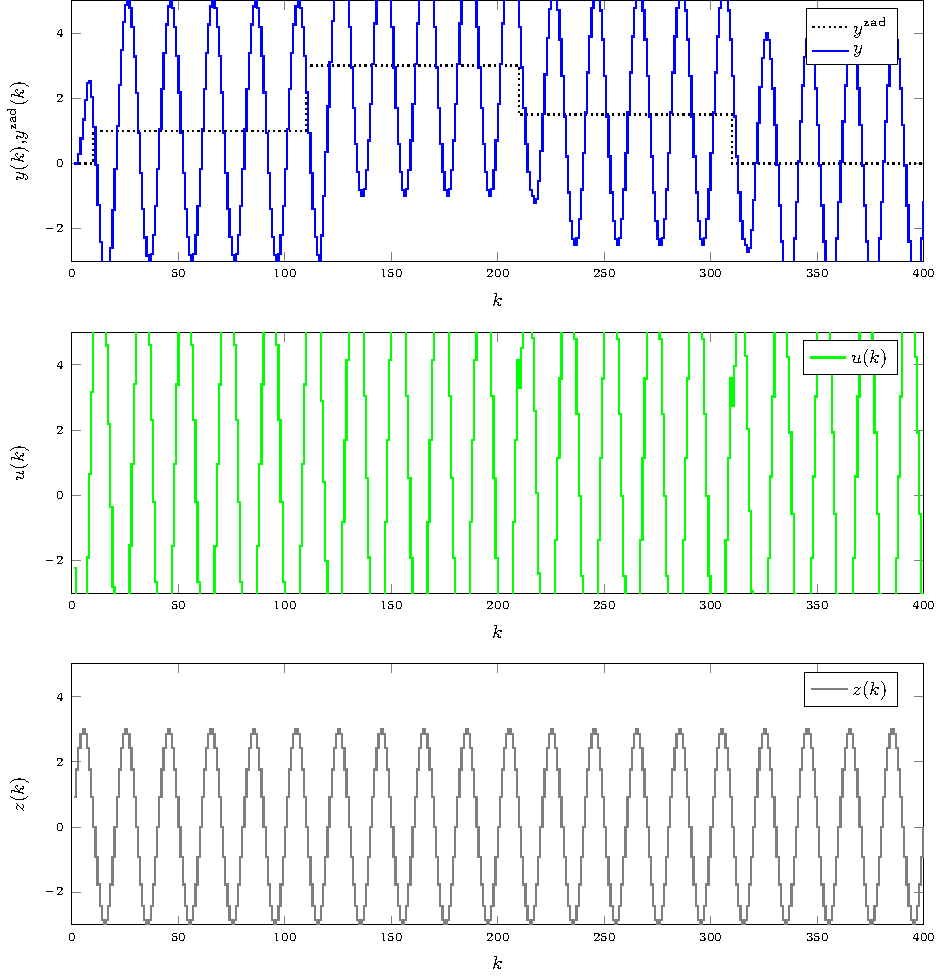
\includegraphics[width=\paperwidth]{data/exercise_6/Desired_output_plot_iter_01_ampl_3_freq_0.1_Dz_20_error_3205.4653.pdf}}
\caption{amplitude=3, freq=0.1, Dz=20, error=3205.4653}
\label{Desired_output_plot_iter_01_ampl_3_freq_0.1_Dz_20_error_3205.4653}
\end{figure}
\end{center}
\begin{center}
\begin{figure}[H]
\makebox[\textwidth]{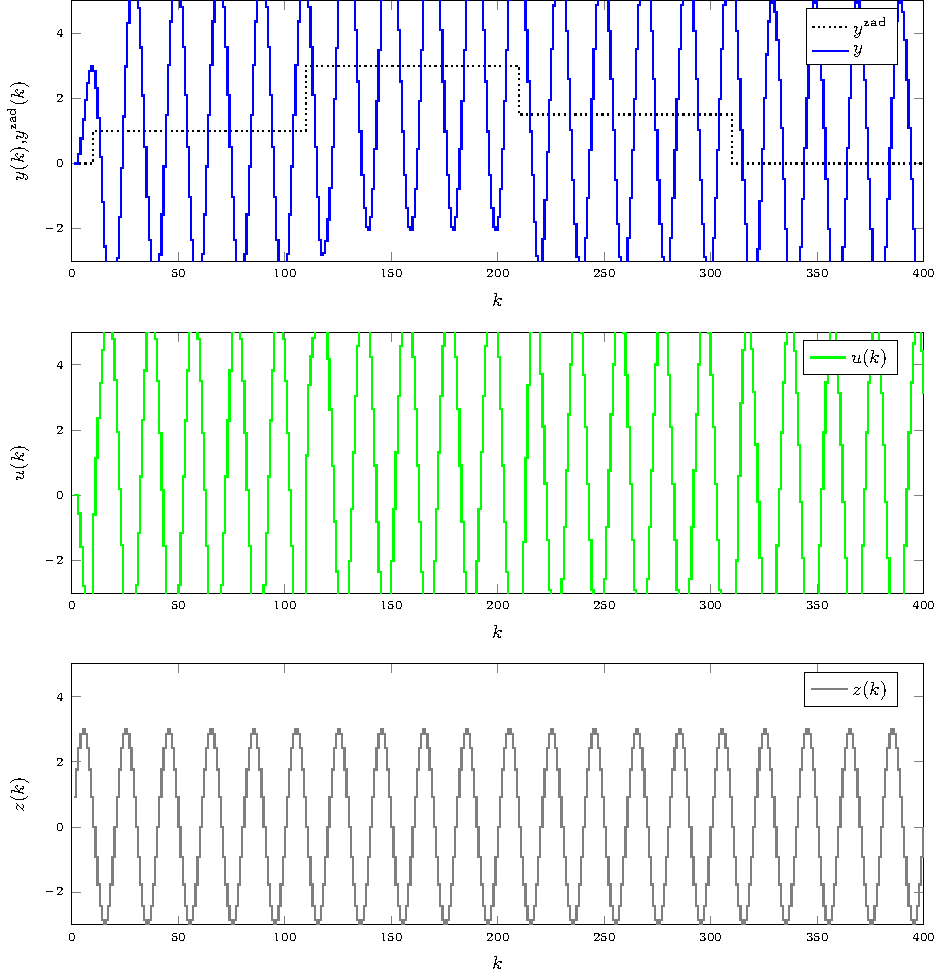
\includegraphics[width=\paperwidth]{data/exercise_6/Desired_output_plot_iter_02_ampl_3_freq_0.1_Dz_0_error_5112.5582.pdf}}
\caption{amplitude=3, freq=0.1, Dz=0, error=5112.5582}
\label{Desired_output_plot_iter_02_ampl_3_freq_0.1_Dz_0_error_5112.5582}
\end{figure}
\end{center}
\begin{center}
\begin{figure}[H]
\makebox[\textwidth]{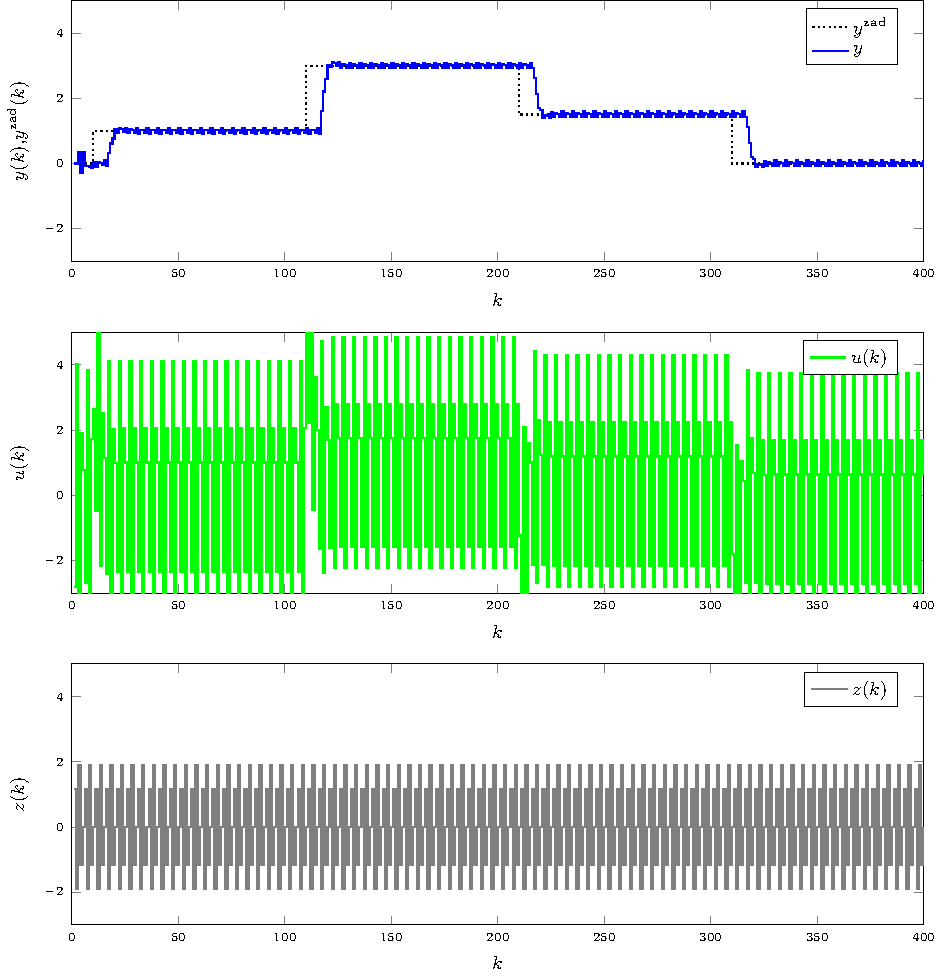
\includegraphics[width=\paperwidth]{data/exercise_6/Desired_output_plot_iter_03_ampl_2_freq_0.8_Dz_20_error_75.3829.pdf}}
\caption{amplitude=2, freq=0.8, Dz=20, error=75.3829}
\label{Desired_output_plot_iter_03_ampl_2_freq_0.8_Dz_20_error_75.3829}
\end{figure}
\end{center}
\begin{center}
\begin{figure}[H]
\makebox[\textwidth]{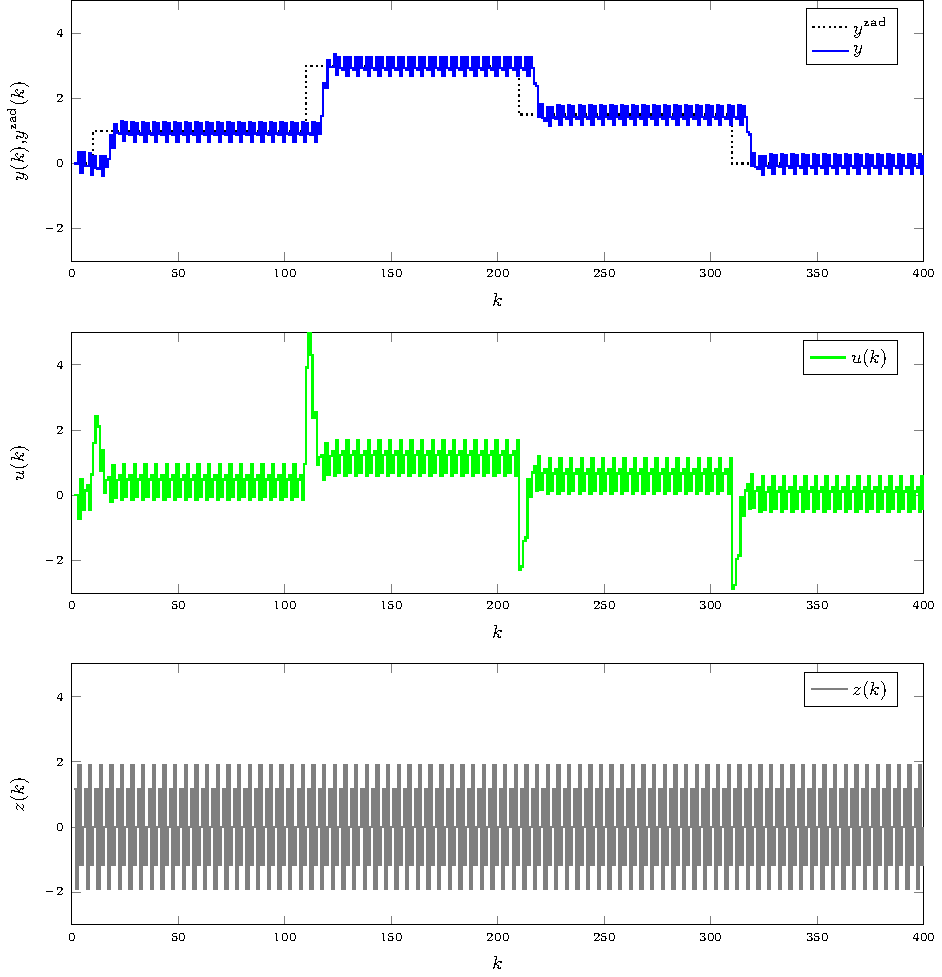
\includegraphics[width=\paperwidth]{data/exercise_6/Desired_output_plot_iter_04_ampl_2_freq_0.8_Dz_0_error_95.3365.pdf}}
\caption{amplitude=2, freq=0.8, Dz=0, error=95.3365}
\label{Desired_output_plot_iter_04_ampl_2_freq_0.8_Dz_0_error_95.3365}
\end{figure}
\end{center}
\begin{center}
\begin{figure}[H]
\makebox[\textwidth]{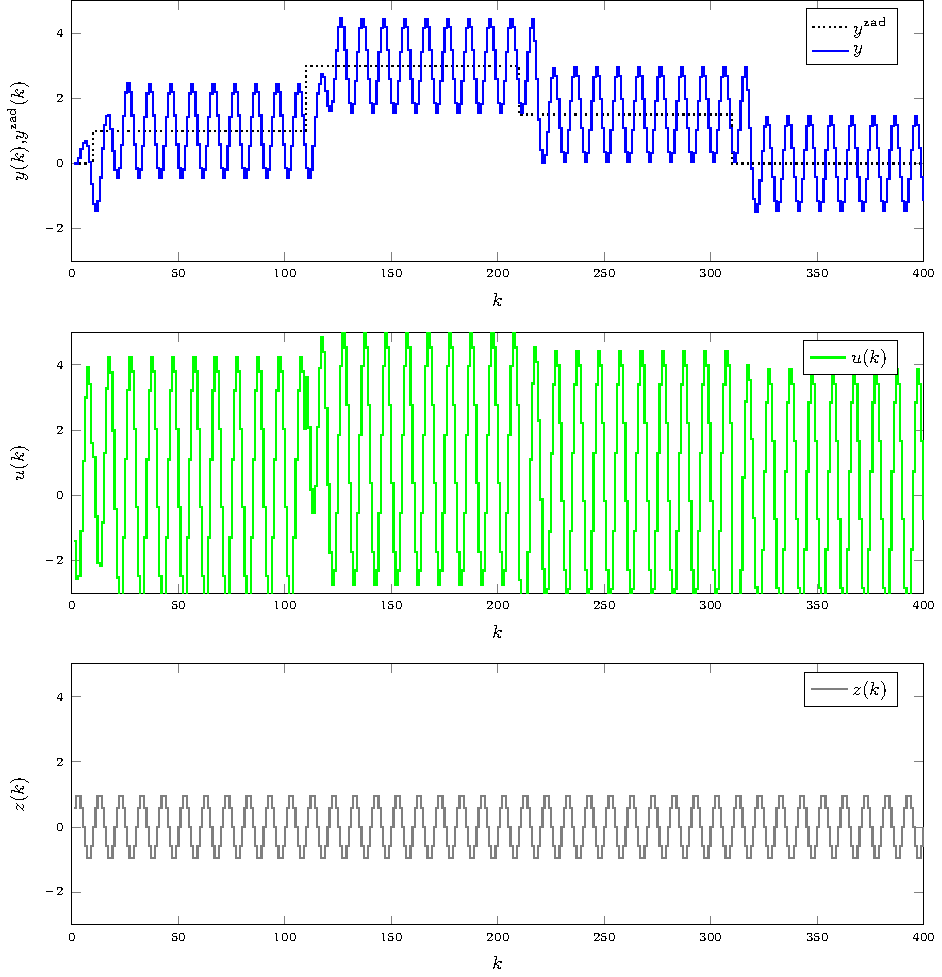
\includegraphics[width=\paperwidth]{data/exercise_6/Desired_output_plot_iter_05_ampl_1_freq_0.2_Dz_20_error_481.7742.pdf}}
\caption{amplitude=1, freq=0.2, Dz=20, error=481.7742}
\label{Desired_output_plot_iter_05_ampl_1_freq_0.2_Dz_20_error_481.7742}
\end{figure}
\end{center}
\begin{center}
\begin{figure}[H]
\makebox[\textwidth]{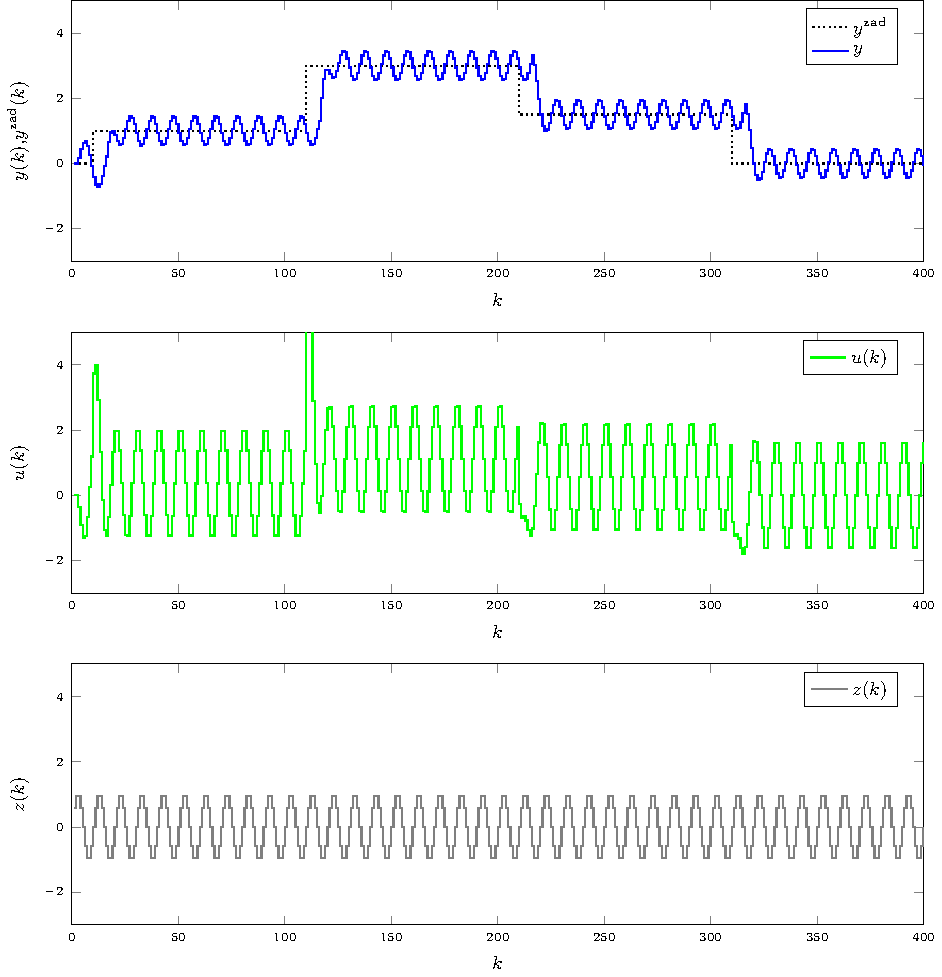
\includegraphics[width=\paperwidth]{data/exercise_6/Desired_output_plot_iter_06_ampl_1_freq_0.2_Dz_0_error_119.0913.pdf}}
\caption{amplitude=1, freq=0.2, Dz=0, error=119.0913}
\label{Desired_output_plot_iter_06_ampl_1_freq_0.2_Dz_0_error_119.0913}
\end{figure}
\end{center}
\begin{center}
\begin{figure}[H]
\makebox[\textwidth]{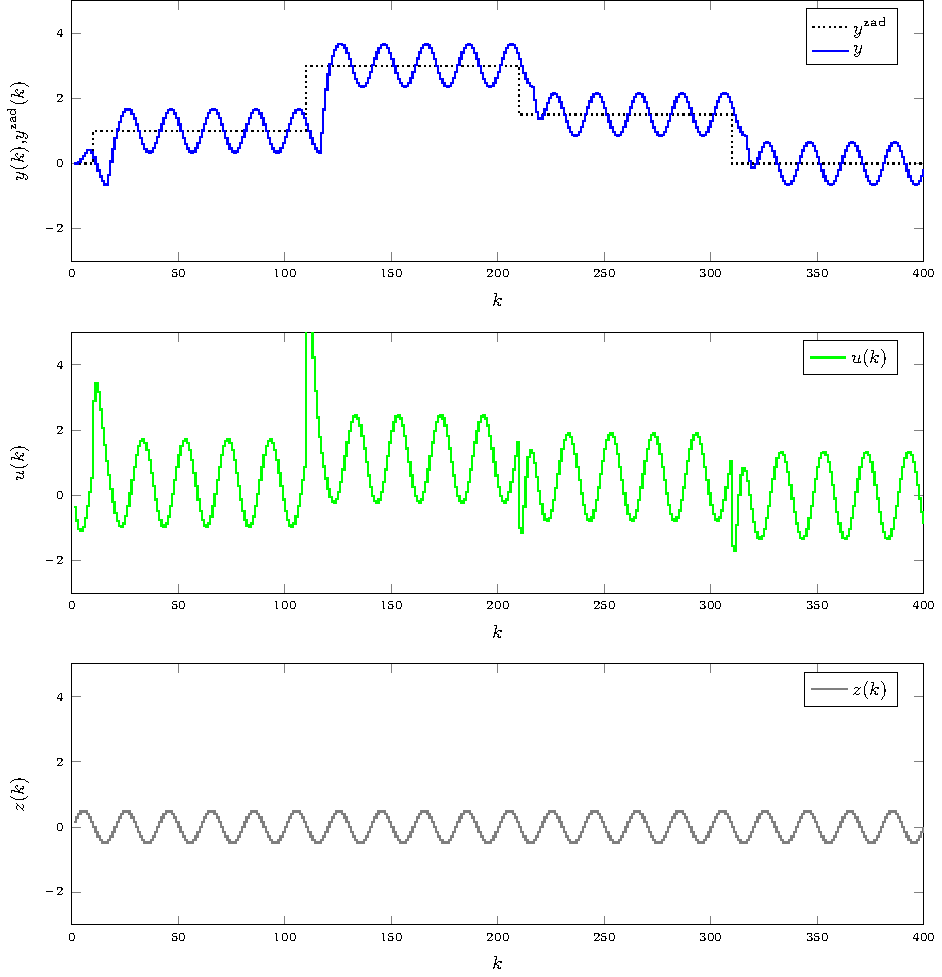
\includegraphics[width=\paperwidth]{data/exercise_6/Desired_output_plot_iter_07_ampl_0.5_freq_0.1_Dz_20_error_160.3299.pdf}}
\caption{amplitude=0.5, freq=0.1, Dz=20, error=160.3299}
\label{Desired_output_plot_iter_07_ampl_0.5_freq_0.1_Dz_20_error_160.3299}
\end{figure}
\end{center}
\begin{center}
\begin{figure}[H]
\makebox[\textwidth]{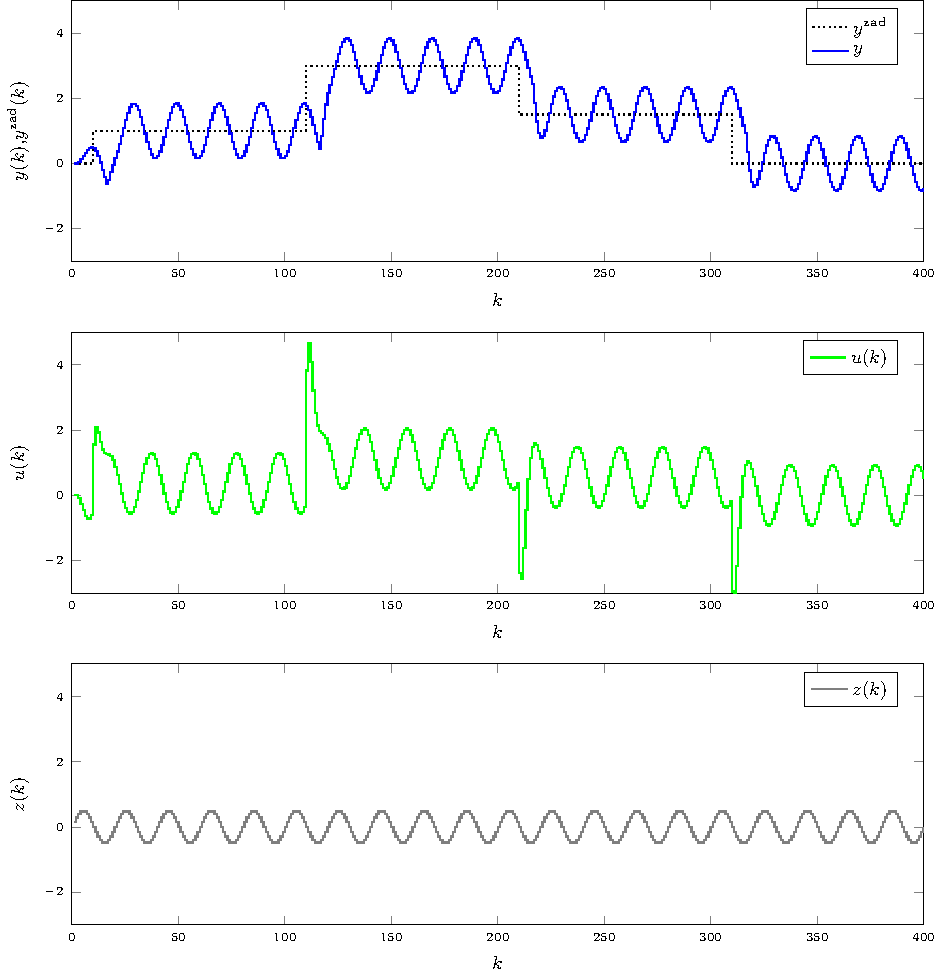
\includegraphics[width=\paperwidth]{data/exercise_6/Desired_output_plot_iter_08_ampl_0.5_freq_0.1_Dz_0_error_215.3014.pdf}}
\caption{amplitude=0.5, freq=0.1, Dz=0, error=215.3014}
\label{Desired_output_plot_iter_08_ampl_0.5_freq_0.1_Dz_0_error_215.3014}
\end{figure}
\end{center}

Jak mo�na zauwa�y�, r�nica w jako�ci regulacji na podstawie przebieg�w z i bez uwzgl�dniania sygna�u zak��caj�cego przez algorytm DMC przy obliczaniu sygna�u steruj�cego jest znacz�ca i tym wi�ksza, czym wy�sza jest amplituda sinusoidy zak��caj�cej.
\section{Charakterystyka statyczna}

Na pierwszy rzut oka stanowisko Inteco mo�na uzna� za obiekt $3 \times 3$. Chwila refleksji uzmys�awia jednak, �e nie wszystkie wej�cia maj� wp�yw na wszystkie wyj�cia. Na przyk�ad rozszczelnienie zaworu poni�ej zbiornika dolnego nie wp�ywa na poziom wody w~zbiorniku g�rnym. Zadanie 7 postawi�o przed nami problem zbadania charakterystyki statycznej obiektu. W~przypadku og�lnego obiektu $3 \times 3$ by�oby to niebagatelne zadania. Wymaga�o by ono najpewniej zbadania stan�w ustalonych wyj�� w~pewnym sze�cianie z~przestrzeni stan�w ustalonych sygna��w wej�ciowych. Dla kraw�dzi takiego sze�cianu ekstrapolowanej z~$n$ punkt�w ($n$ pomiar�w) oznacza�oby to konieczno�� wykonania $n^3$ ekperyment�w! Innym podej�ciem, przy za�o�eniu, �e obiekt jest, przynajmniej w~przybli�eniu, liniowy by�oby zebranie odpowiedzi skokowych dla ka�dego toru wej�cia-wyj�cia i~identyfikacja na ich podstawie macierzy transmitancji obiektu. Z~macierzy tej mo�naby z~kolei w~spos�b analityczny wyznaczy� charakterystyk� statyczn�.


Problem ten mo�na jednak w~znakomitym stopniu upro�ci�, je�eli we�mie si� pod uwag� pewne charakterystyczne cechy obiektu. Za��my, �e obiekt znajduje si� w~stanie ustalonym \footnote{Tak jak w~tre�ci zadania zak�adamy, �e dop�yw do g�rnego zbiornika jest sta�y, �~manipulujemy jeydnie stopniem rozszczelnienia zawor�w}. Je�eli zmienimy stopie� otwarcia zaworu pod zbiornikiem g�rnym, to poziom wody zmieni si� oczywi�cie chwilowo we wszystkich zbiornikach \footnote{Ze zbiornika g�rnego zacznie wyp�ywa� wi�cej wody, zatem wi�cej wody wpadna� b�dzie do zbiornika �rodkowego, przez co zwi�kszy si� w~nim ci�nienie hydrostatyczne. Poskutkuje to zmian� wyp�ywu z~tego zbiornika i~zaj�ciem podobych zmian w~zbiorniku dolnym.}. Zauwa�my jednak, �e po pewnym czasie poziom wody w~zbiorniku g�rnym ustali si� na pewnym poziomie. Je�eli poziom b�dzie utrzymywany, a~dop�yw do zbiornika g�rnego sta�y to b�dzie to znaczy�, �e wy�ywa z niego ta sama ilo�� wody, co przed zmian� pozycji zaworu. Co za tym idzie, poziomy w~pozosta�ych zbiornikach r�wnie� wr�c� do stanu pierwotnego. Rozumowanie to mo�na uog�lni� na wszystkie zbiorniki. 

\vskip 1cm
\begin{figure}[H]
    \centering
	\begin{tikzpicture}
		\begin{axis}[
			width=0.75\textwidth,
			height=0.45\textwidth,
			xmin=-1,xmax=1,ymin=-2,ymax=22,
			xlabel={$u$},
			ylabel={$y$},
			xtick={-1, -0.6, -0.2, 0.2, 0.6, 1},
			ytick={-2, 2, 6, 10, 14, 18, 22},
			legend pos=north west,
			y tick label style={/pgf/number format/1000 sep={,}},
		]
		\addplot[smooth, blue]   file {data/exercise_7/static_high.txt};
		\addplot[smooth, red]    file {data/exercise_7/static_medium.txt};
		\addplot[smooth, green]  file {data/exercise_7/static_low.txt};
		\legend{$U1-Y1$, $U2-Y2$, $U3-Y3$}
	\end{axis}
	\end{tikzpicture}
    \caption{Charakterystyki statyczne poszczeg�lnych zbiornik�w stanowiska Inteco}
    \label{inteco_static}
\end{figure}
\vskip 1cm

Spostrze�enie to nasuwa bardzo praktyczny wniosek: patrz�c jedynie z~punktu widzenia stan�w ustalonych, stanowisko Inteco mo�na traktowa� jako trzy obiekty wymiaru $1 \times 1$. Co za tym idzie, do okre�lenia charakterystyki statycznej obiektu wystarczaj�ce jest przeprowadzenie $n$ eksperyment�w dla ka�dej pary wej�cie-wyj�cie. Eksperymenty takie zosta�y przeprowadzone, a~ich wyniki przedstawiono rys. \ref{inteco_static}. Pomiary na ka�dym torze wykonywane by�y w~przedziale sterowa� $<0; 1>$ z~krokiem $0.1$. Jak wida�, tory s� silnie nieliniowe. Charakterystyki mog� by� przybli�on� relacj� $\overline{y}(\overline{u}) ~ \sqrt{\overline{u}}$, co zgadza si� z~przewidywaniami teoretycznymi. Zgodnie z~tre�ci� zadan projektowych sterowanie obiektem powinno by� ograniczone do warto�ci zadanych z~przedzia�u $<10; 15>$. W~tym zakresie mo�na z~powodzeniem przybli�y� chcarakterystyki funkcjami liniowymi, co uzasadnia u�ycie klasycznego regulatora PID do sterowania obiektem.

\end{document}
